\documentclass[12pt]{article}

    %packages
    \usepackage{comment}
    \usepackage{graphicx}
        \graphicspath{{./images/}}
    \usepackage[backend=biber, style=ieee]{biblatex}
        \addbibresource{references.bib}
    \usepackage{caption}
    \usepackage{subcaption}
    \usepackage{fancyhdr}
    \renewcommand*{\familydefault}{\sfdefault}
    \usepackage{geometry}
    \usepackage{lmodern}
    \usepackage{setspace}
    \usepackage{xcolor}
    \usepackage{tikz}
    \usepackage{amsmath}

    \usepackage{hyperref}
        \hypersetup{colorlinks=false, pdfnewwindow=true}

    %colors
    \definecolor{purple}{RGB}{80, 0, 100}

%Creates a footer for normal and chapter pages
    \pagestyle{fancy}
    \fancyhf{}
    \lfoot{{\the\year} Jose Antonio Lara Perez}
    \rfoot{Page \thepage}

\begin{document}
%Title page -------------------------------------------
    \begin{titlepage}
        \thispagestyle{empty}
        \newgeometry{left=2cm, right=1cm, top=2cm, bottom=2cm}
        \begin{tikzpicture}[overlay, fill opacity=0.8]
            \rotatebox{-40}{\fill[purple](11.8, -23) rectangle (35, 20);}
        \end{tikzpicture}
        \begin{spacing}{1.5}
            {\Huge \bfseries \noindent UNIT 3 \& 4 PROJECT REPORT}\\[15pt]
            {\LARGE ROBOTS KINEMATICS AND DYNAMICS}\\
            {\large Computational Robotics Engineering}\\[1.5cm]
        \end{spacing}
        \begin{minipage}{2cm}
            \hspace{0.5cm} \rotatebox{90}{\Large UNIVERSIDAD POLIT\'ECNICA DE YUCAT\'AN}    
        \end{minipage}
        \hfill
        \begin{minipage}{5cm}
            \begin{spacing}{4}
                {\fontsize{70}{70}\selectfont \bfseries \color{white}2\\0\\2\\4}
            \end{spacing}
        \end{minipage}
        \vfil
        \begin{flushleft}
            \begin{minipage}{6cm}
                {\color{white}
                \textbf{Name: }Jos\'e Antonio Lara P\'erez\\
                \textbf{Professor: }Jos\'e Rodr\'iguez Torres\\
                \textbf{Group: }7B\\
                \textbf{Date: }\today}
            \end{minipage}
            \hfill
            \begin{minipage}{8cm}
                %Add image manually
                
\includegraphics[width = 3in]{Upy-logo-large.png}
            \end{minipage}
        \end{flushleft}

    \end{titlepage}
%END---------------------------------------------------

%Body of the document
    \section{Introduction}

    \section{Development}
    For this project I have select a 3-DoF RPP Robot. This robot have a rotative link and 2 prismatic links, you can
    see thie robot on figure \ref{fig:robot}.
    \begin{figure}[h]
        \centering
        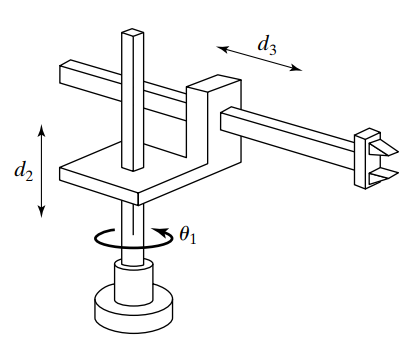
\includegraphics[width = 3in]{RPP.png}
        \caption{Image of the RPP Robot.}
        \label{fig:robot}
    \end{figure}

    \begin{table}[h]
        \begin{center}
            \begin{tabular}{c c c c c c}
                \hline
                $i-1$ & $i$ & $a_{i-1}$ & $\alpha_{i-1}$ & $d_i$ & $\theta_i$\\
                \hline
                0 & 1 & 0 & 0 & 0 & $\theta_1$\\
                1 & 2 & 0 & 0 & $d_2$ & 0\\
                2 & 3 & L2 & $\pi / 2$ & $d_3$ & 0\\
                \hline
            \end{tabular}
        \end{center}
        \captionof{table}{DH Table}
        \label{table:DH_table}
    \end{table}
        \subsection{Direct Kinemtics}
        Once we have solve the homogene transform of the robot, we can obtain the equation of the direct kinematics.
        This equations will help us to determine where is located the end effector with respect of the base.
        
    \begin{equation}
	    x = L_2 * cos(\theta_1) + d_3 * sin(\theta_1)
        \label{eq:x}
    \end{equation}
    \begin{equation}
        y = L_2 * sin(\theta_1) - d_3 * cos(\theta_1) 
        \label{eq:y}
    \end{equation}
    \begin{equation}
        z = d_2
        \label{eq:z}
    \end{equation} 

        As  we can observe, the reachability of this robot is determined by $d_2$, $d_3$ and $\theta_1$.
        \subsection{Inverse Kinemtics}
        Now that we have the equations \ref*{eq:x}, \ref*{eq:y} and \ref*{eq:z}. We need to solve for $d_2$, $d_3$ and $\theta_1$.
        I first used the algebraic approach, that const on elevate both $x$ and $y$ to the second power and equal them to their corresponding equations.
        Yo can see this process in 


    \section{Simulation}
    You can see the code for this simulation on appendix \ref{sec:matlabcode}
    \section{Conclusion}

%Bibliography------------------------------------------
    \pagebreak
    \section*{References}
    \addcontentsline{section}{References}
    \printbibliography
%END---------------------------------------------------

%Appendix if required
    \pagebreak
    \appendix
    \section{Matlab code}
    Here is the code use for the simulation file on Matlab

    %Copy code and paste here

    \label{sec:matlabcode}
    \section{Inverse Kinematics procedure}
    From equations \ref{eq:x}, and \ref{eq:y}, we can elevate both equation to the second power:
    \begin{equation}
        \begin{split}
        x^2 + y^2 & = (L_2 * cos(\theta_1) + d_3 * sin(\theta_1))^2 + (L_2 * sin(\theta_1) - d_3 * cos(\theta_1))^2 \nonumber \nonumber \\
	     & = L_2^2 * cos(\theta_1)^2 + 2*L_2*d_3*cos(\theta_1)*sin(\theta_1) + d_3^2 * sin(\theta_1)^2 \nonumber \\
        & + L_2^2 * sin(\theta_1)^2 - 2*L_2*d_3*cos(\theta_1)*sin(\theta_1) + d_3^2 * cos(\theta_1)^2 \nonumber
        \end{split}
    \end{equation}
    Reducing terms of the equation, we get:
    \begin{equation} 
        \begin{split}
	        x^2 + y^2 = L_2^2 + d_3^2 \nonumber
        \end{split}
    \end{equation}
    Solving for $d_3$, we obtain:
    \begin{equation}
        d_3 = \sqrt{x^2 + y^2 - L_2^2}
    \end{equation}
    


\end{document}